\section{绘图分析}
在绘制图形前,首先让我们对端盖的零件图进行必要的分析。这一过程不仅不会耽误绘图,还能够加速我们的绘图过程,正所谓“磨刀不误砍柴功”。通过对图\ref{fig:tiaoyafaduangai}的观察,可以看出主视图清楚的地表达了端盖零件是回转体类的零件,与第\ref{chap:bei}章的杯零件和第\ref{chap:dianpian}章的垫片零件均属于同一类。但端盖零件无论是外形还内部结构均比杯和垫片块零件复杂。而这种复杂性决定了不同建模策略的复杂性,也同时决定了建模效率。因此绘图分析的根本目的是要找出其能够最准确、最简便、最快捷的建模策略,并以此来提升零件的建模效率。

根据第\ref{chap:bei}章的杯零件和第\ref{chap:dianpian}章的垫片零件建模的经验,大致有两种技术路线图可以用于端盖零件的三维建模,即主视图技术路线图和左视图路线图。

\subsection{主视图技术路线}
图\ref{fig:tiaoyafaduangaifront}所示的端盖主视图可由5个不同直径圆柱和6个直径为$\diameter 9$的圆柱组成。然后利用圆柱之间的并、差、交集关系来实现模型的构建。其整个建模过程中需要利用辅助点或线来帮助圆的定位。
\begin{figure}[htbp]
\centering
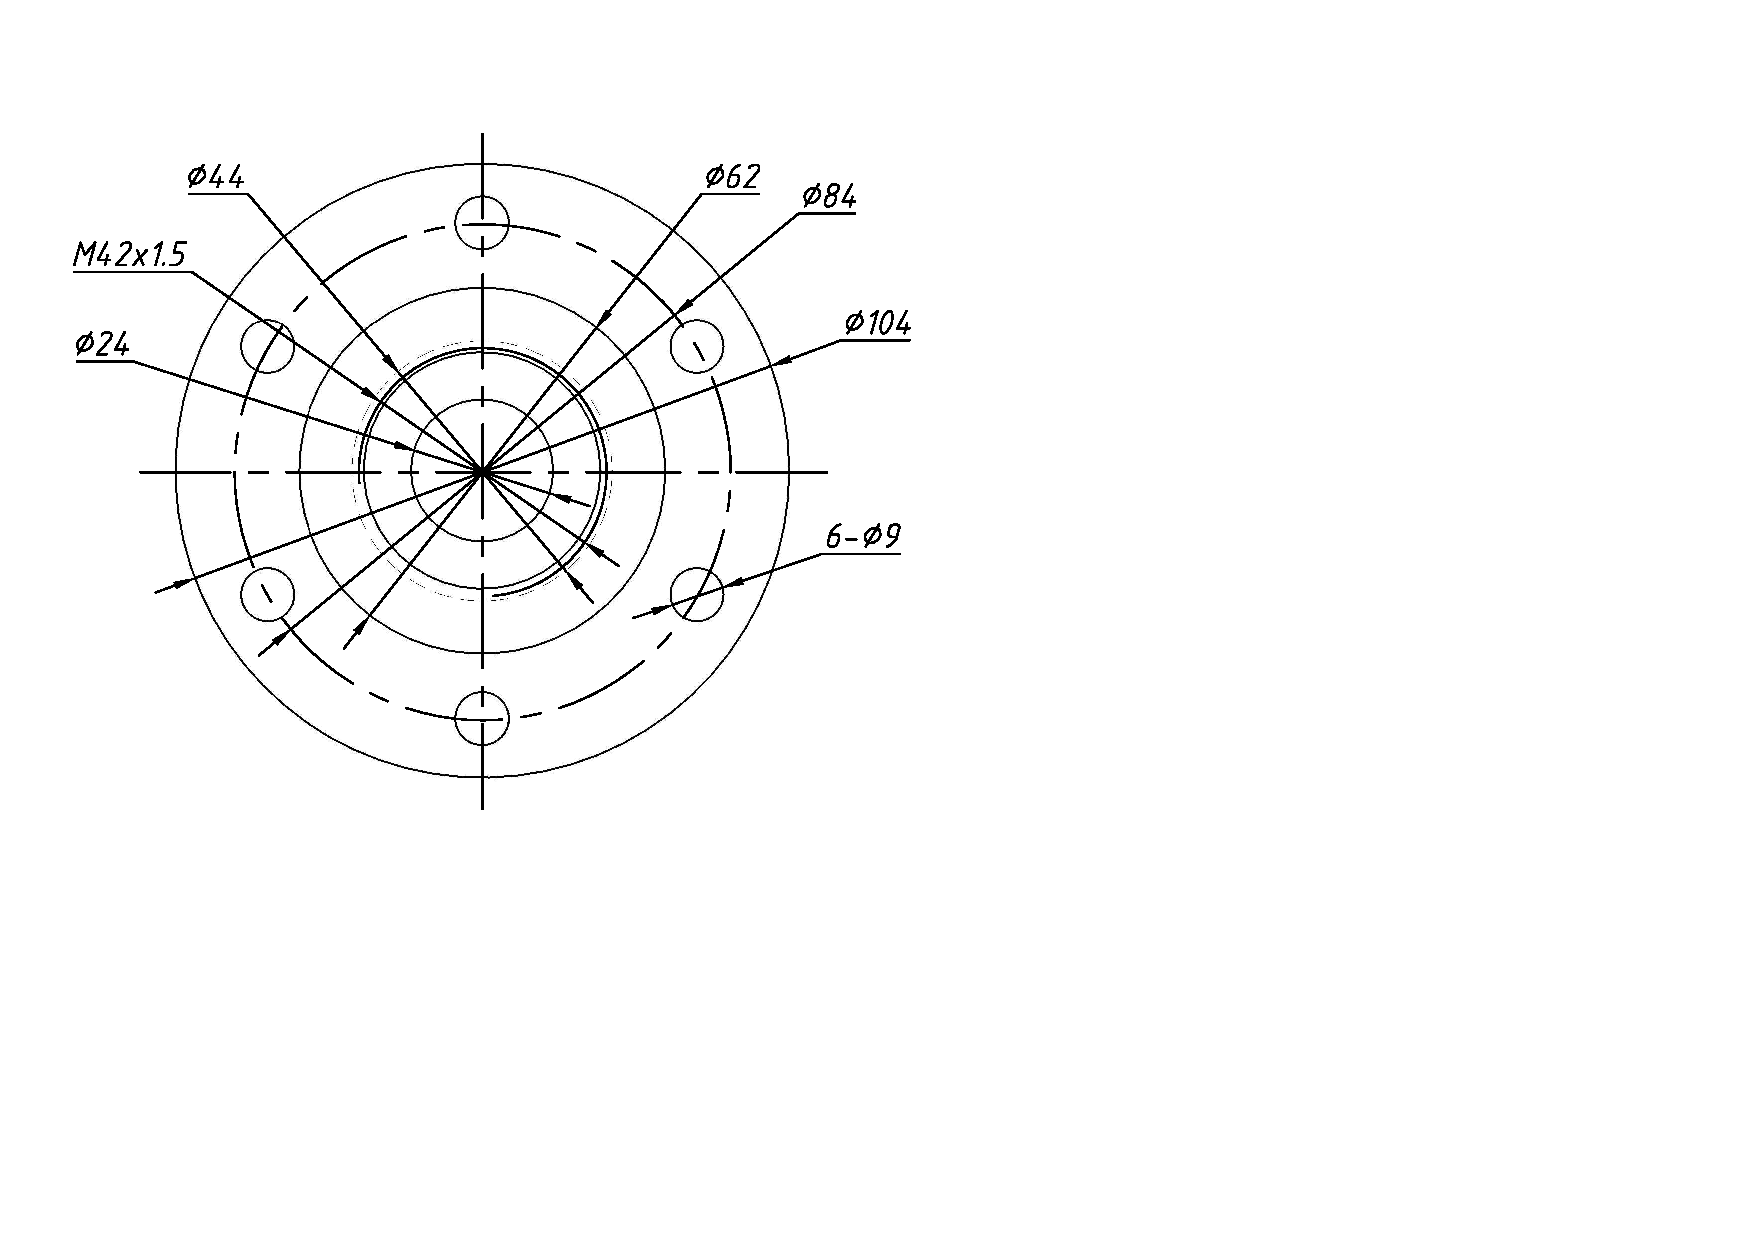
\includegraphics[scale=0.5]{tiaoyafaduangaifront.pdf}
\caption{端盖主视图}\label{fig:tiaoyafaduangaifront}
\end{figure}
\subsection{左视图技术路线}

\endinput